\section{Experiments}
\label{sec:experiments}

\subsection{Dataset}

We evaluate our algorithms using one month (May, 2013) of  New York City's taxi dataset~\cite{nyc}, which contains 39,437 drivers and around 500,000 trips per day. Each ride in the dataset has a pick-up latitude/longitude, a drop-off latitude/longitude and request time. We extracted the road network of New York City from Open Street Map (OSM), which is represented as an undirected graph with 55,957 vertices and 78,597 edges. Subsequently, we mapped the source and destination of each trip to the road network. Similar to~\cite{Huang14}, we maintain a cache for shortest paths between vertices, which means that the shortest path can be found in constant time. Initially, each driver is randomly located on one vertex of the road network. When the vehicle is serving rider requests, we assume it is following the schedule and constantly moving towards the destination.

\subsection{Experimental Methodology}

To evaluate \textbf{LSTM}'s prediction precision, we compare its performance in predicting the transition model to that of \textbf{LORE}~\cite{Zhang14}. LORE models transition probabilities based on their previous locations using Additive Markov Chains.

In our evaluation we used the k-fold cross validation (k=4) method to divide our data into test and train sets and for each fold compared the models built with LSTM and LORE with the actual transition probabilities for the test data. To compare the transition probabilities of the test data to those from the output of the model, we used the \emph{Kullback-Leibler divergence (KLD)} metric \cite{kullback51}. The reason for choosing KLD is that unlike other widely used metrics (e.g. the Jensen-Shanon divergence \cite{Rubner98}), KLD is not symmetric and is best used when measuring how a probability distribution (model output) diverges from an expected probability distribution (test data). With KLD, we measure the divergence of probability distribution $Q$ from $P$ as:
\begin{equation*}
KLD\left(P \middle\| Q\right)=\sum_i P(i) \log \frac{P(i)}{Q(i)}
\end{equation*}
Based on the definition of KLD, the lower the KLD score is, the closer $Q$ is to $P$ where a KLD score of $0$ means that $Q$ and $P$ are equal.

Subsequently, we compare the proposed second-price auction with reserved price scheme (\textbf{SPARP}) with the regular second-price auction scheme (\textbf{SPA}) and the first-price auctions scheme where drivers are not truthful and bid competitively (\textbf{FPACB}). We compare the generated revenue in different pricing mechanisms and also evaluate the effects of bidding competitively on the workers utility in a first-price auction scheme. 

\Cref{tab:params} shows the different values we used for various parameters we used in our experiments (default values are shown in \textbf{bold}). 
\begin{table}[!ht]
	\begin{center}
		\begin{tabular}{|c|c|}
			\hline
			Parameter & Values \\
			\hline \hline
            Grid Size (km) & 1, \textbf{2}, 3, 4, 5 \\ 
			\hline
			Time Slot Size (hour) & 1, \textbf{2}, 3,  4, 5, 6\\ 
			\hline
			Max Wait Time (min) & 3, \textbf{6}, 9, 12, 15, 20 \\ 
			\hline
			\# of Drivers & 1000, 2000, \textbf{5000},  10000, 20000\\ 
			\hline
			Max Passengers & 2, 3, \textbf{4}, 5, 6 \\
			\hline
			Max Allowed Detour & 25\%, \textbf{50\%}, 75\%, 100\%\\
			\hline
		\end{tabular}
		\caption{Parameters for Algorithm Comparison}
		\label{tab:params}
	\end{center}
\end{table}

For the pricing model, the default configurations are:
\begin{align*}
F(\phi_r) =& 2 \times \phi_r\\
\forall r, \lambda_r(\Delta_r) = & 1 - \Delta_r^2\\
\forall d, \theta_d(l) = & 1.5 * l
\end{align*}

\subsection{Prediction Model}

In the first set of experiments, we compared the prediction precision of LSTM to that of LORE. \Cref{fig:var_time,fig:var_cell} depict the KLD scores of LSTM and LORE for varying time slots and cell sizes, respectively. The reason LSTM predicts transition probabilities better than LORE is because different topics can capture transition patterns that are observed in the training data. To better illustrate the improvements of LSTM over LORE, in \Cref{fig:klddiff} we did a pairwise comparison between the KLD scores of LSTM and LORE. Each bar shows the percentage of improvement we observed for each (\emph{Cell Size}, \emph{Time Slot Size}) pair. As the number of regions and time slots increase (i.e., smaller cell and time slot sizes), more patterns can be observed in the data and yielding better accuracy for LSTM.
\begin{figure}[!ht]
    \centering
    \subfigure[\small{Varying Time Slot Size (h)}]{
        \label{fig:var_time}
        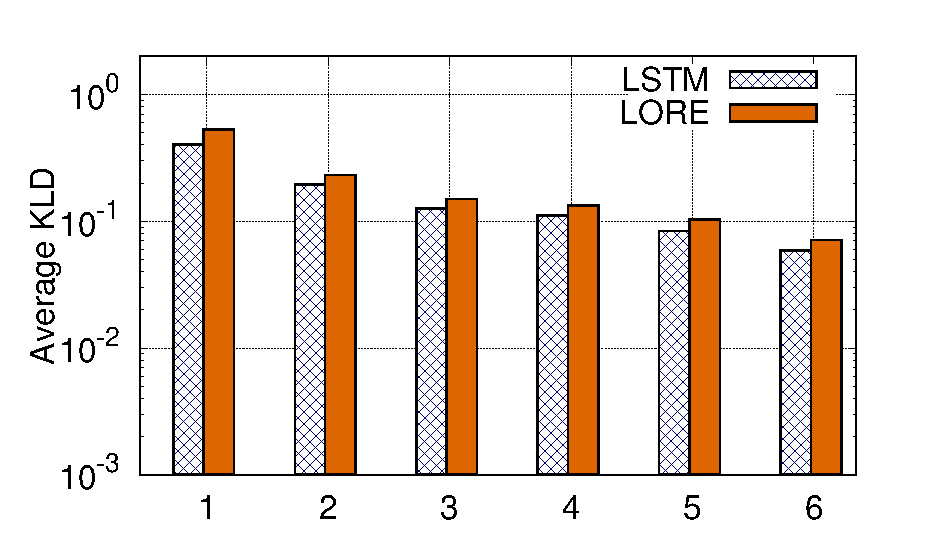
\includegraphics[width = 0.47\columnwidth]{fig/modelhs}
    }
    \subfigure[\small{Varying Cell Size (km)}]{
        \label{fig:var_cell}
        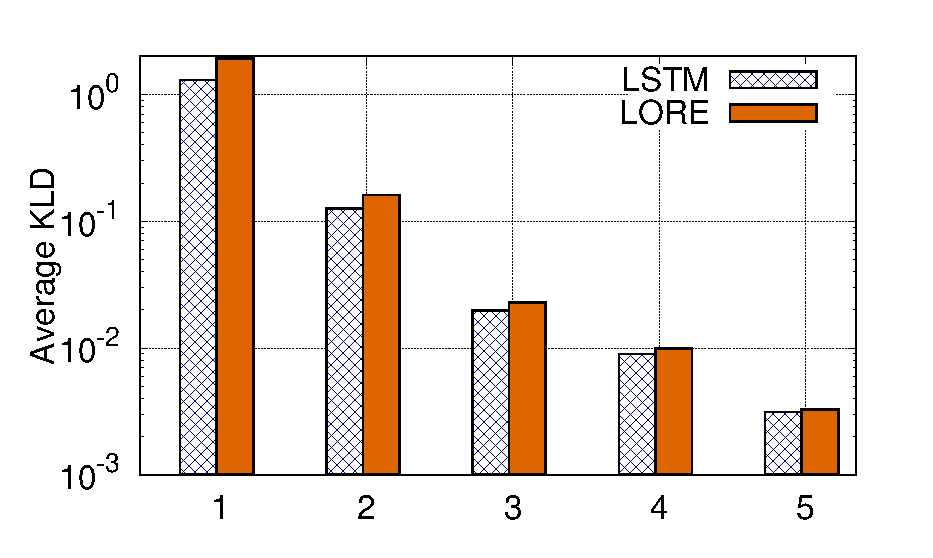
\includegraphics[width = 0.47\columnwidth]{fig/modelcs}
    }
    \caption{Comparing Precision of LSTM Vs LORE}
    \label{fig:defaults}
\end{figure}

\begin{figure}[!ht]
	\centering
	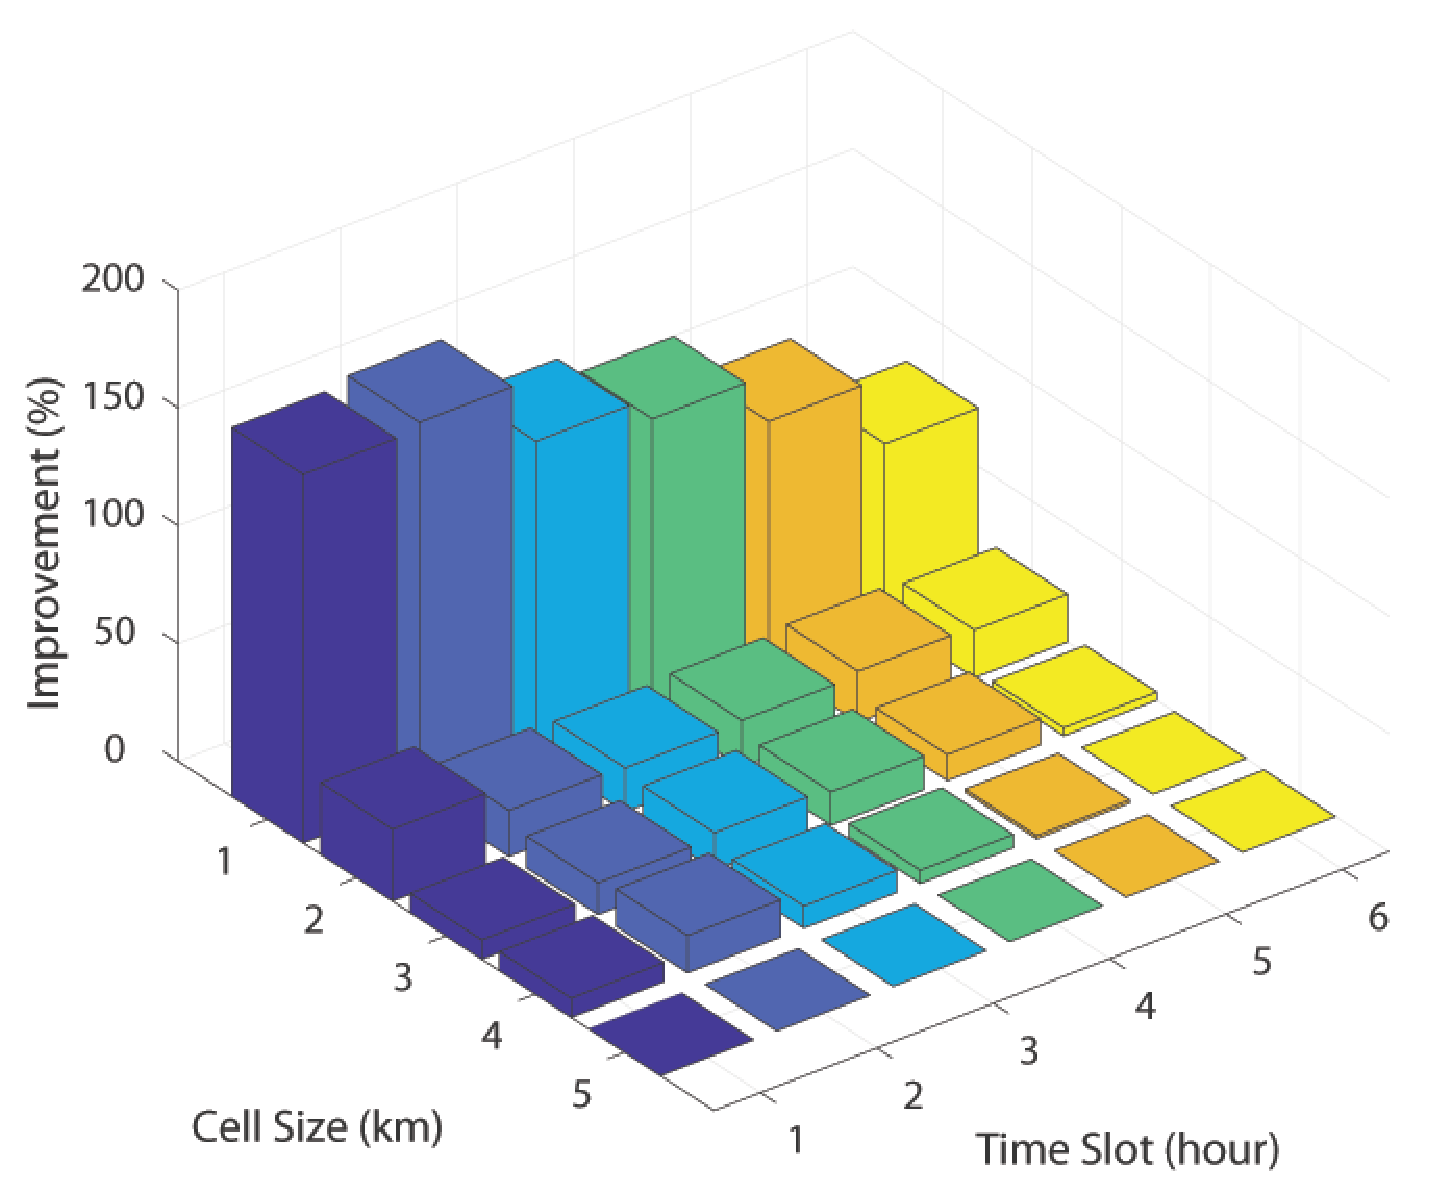
\includegraphics[width=0.75\columnwidth]{fig/klddiff}
	\caption{LSTM Vs LORE - Varying Cell \& Time Slot Size}\label{fig:klddiff}
% * <masghari@usc.edu> 2017-06-19T22:24:31.560Z:
%
% ^.
% * <masghari@usc.edu> 2017-06-19T22:24:26.860Z:
%
% ^.
\end{figure}

\subsection{Pricing Mechanism}

In the next set of experiments, we compare the generated revenue of each pricing mechanism. Towards this end, we compute the fares and cost of the drivers based on \Cref{eq:fare,eq:cost}. We compare the generated revenue under different scenarios by varying the parameters in \Cref{tab:params}.

As depicted in \Cref{fig:rev}, SPA generates less revenue than FPACB since the platform will only receive a profit for each request that's equal to the second highest bid. However, by introducing the \emph{reserved price} in SPARP, we manage the losses in SPA. Furthermore, because the drivers do not bid truthfully in FPACB, in most cases, SPARP slightly generates more revenue than FPACB. To better show the difference between the revenue of each mechanism under different configurations, in \Cref{fig:revdiff} we show the relative difference of both SPA and SPARP when compared to FPACB. 

\begin{figure}[h]
    \centering
    \subfigure[\small{Maximum Wait Time}]{
        \label{fig:mwt2rev}
        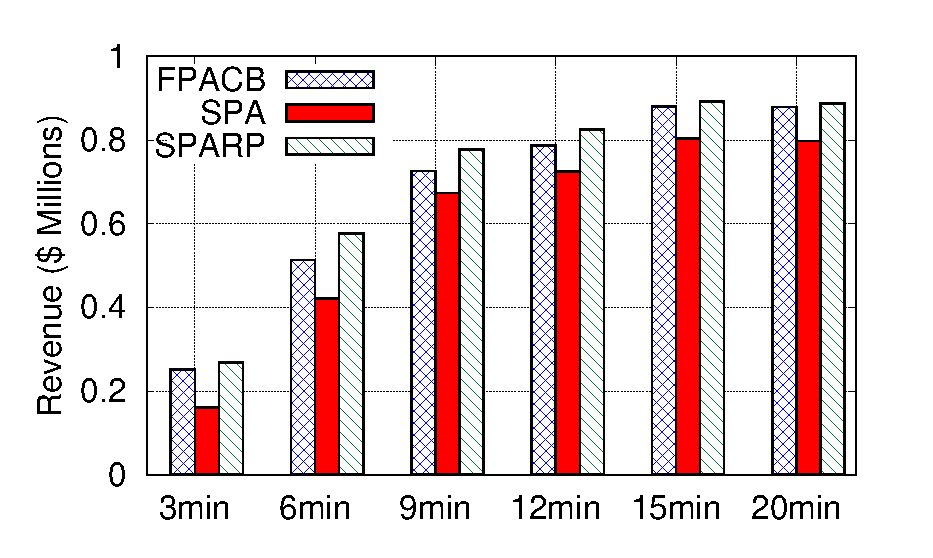
\includegraphics[width = 0.47\columnwidth]{fig/mwt2rev}
    }
    \subfigure[\small{Number of Drivers}]{
        \label{fig:nd2rev}
        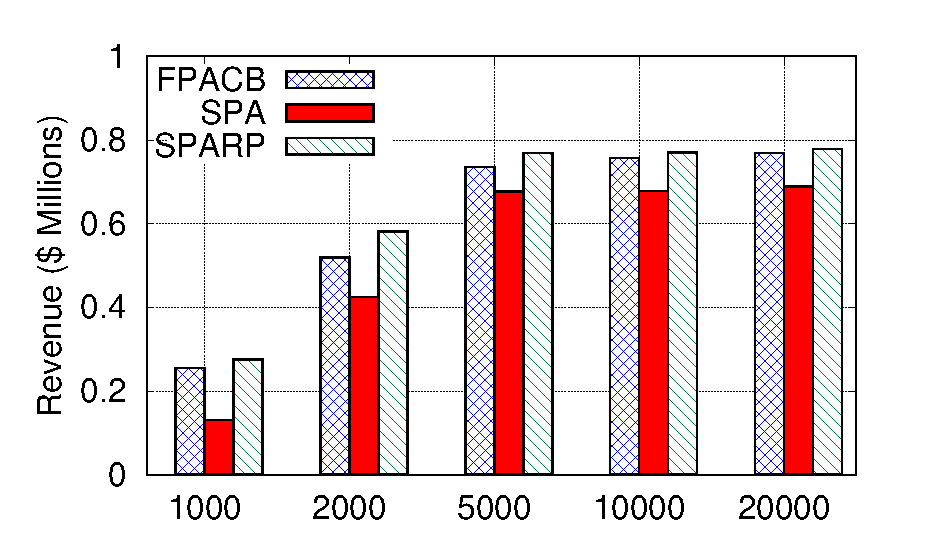
\includegraphics[width = 0.47\columnwidth]{fig/nd2rev}
    }
    \subfigure[\small{Maximum Passengers}]{
        \label{fig:mp2rev}
        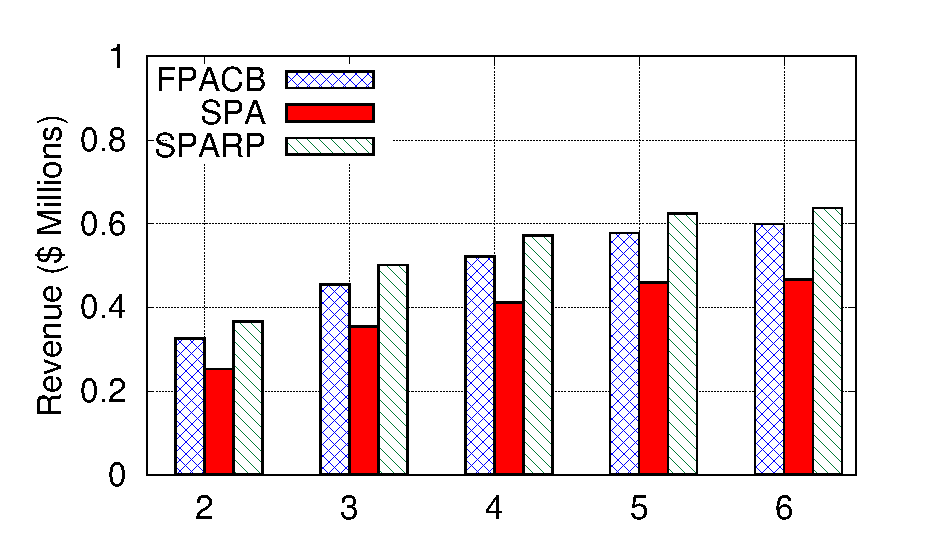
\includegraphics[width = 0.47\columnwidth]{fig/mp2rev}
    }
    \subfigure[\small{Maximum Allowed Detour}]{
        \label{fig:mad2rev}
        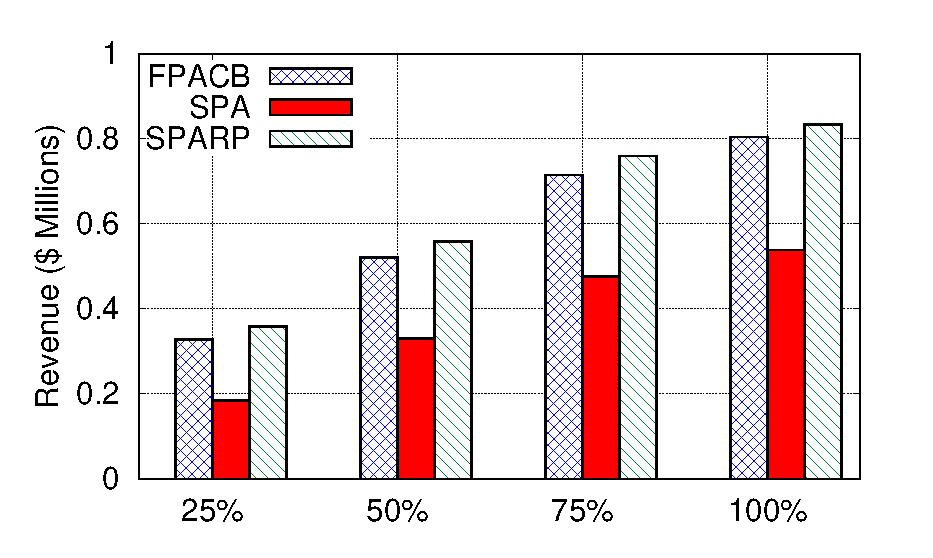
\includegraphics[width = 0.47\columnwidth]{fig/mad2rev}
    }
    \caption{Comparing Revenue of Different Mechanisms}
    \label{fig:rev}
\end{figure}

\begin{figure}[h]
    \centering
    \subfigure[\small{Maximum Wait Time}]{
        \label{fig:mwt2revdiff}
        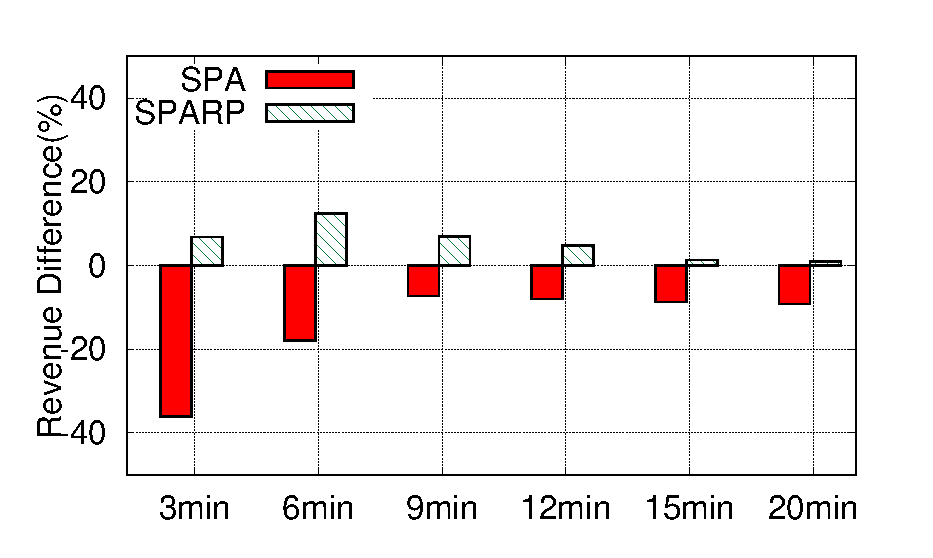
\includegraphics[width = 0.47\columnwidth]{fig/mwt2revdiff}
    }
    \subfigure[\small{Number of Drivers}]{
        \label{fig:nd2revdiff}
        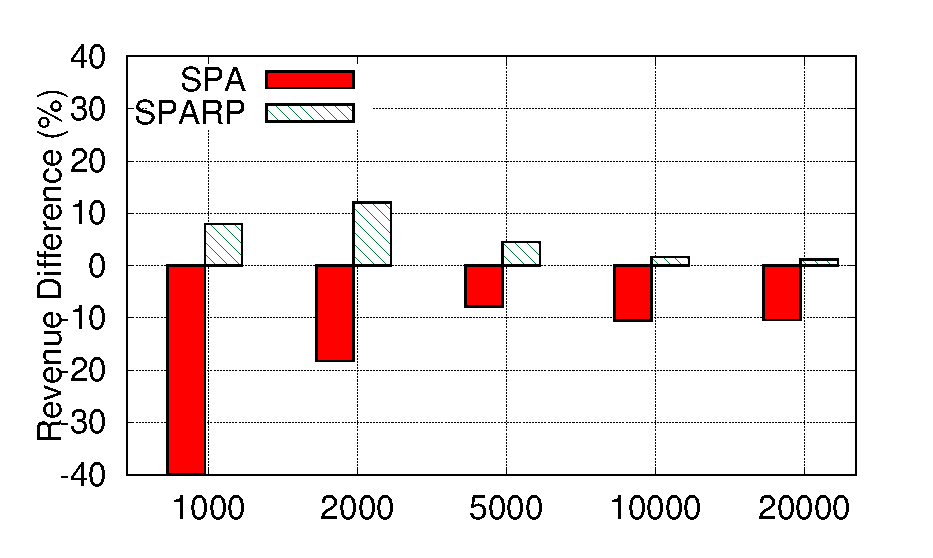
\includegraphics[width = 0.47\columnwidth]{fig/nd2revdiff.eps}
    }
    \subfigure[\small{Maximum Passengers}]{
        \label{fig:mp2revdiff}
        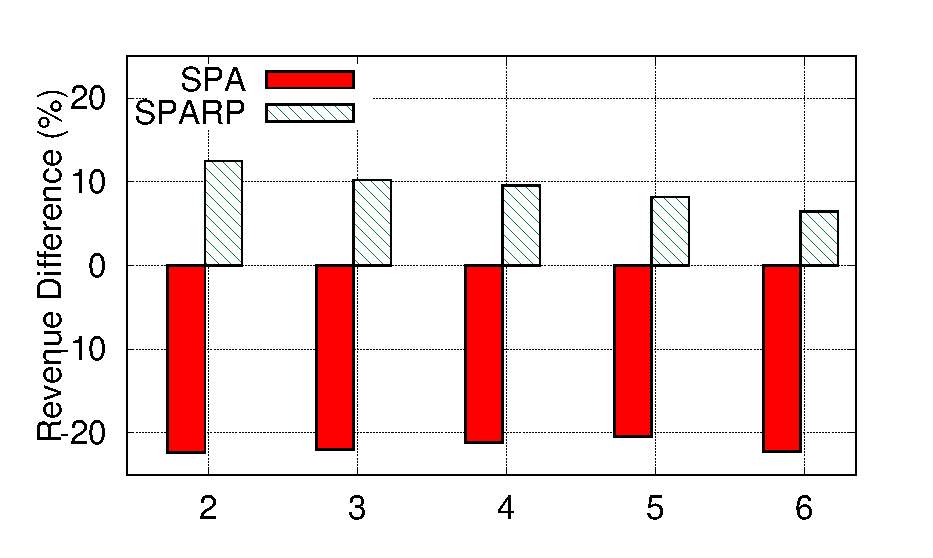
\includegraphics[width = 0.47\columnwidth]{fig/mp2revdiff}
    }
    \subfigure[\small{Maximum Allowed Detour}]{
        \label{fig:mad2revdiff}
        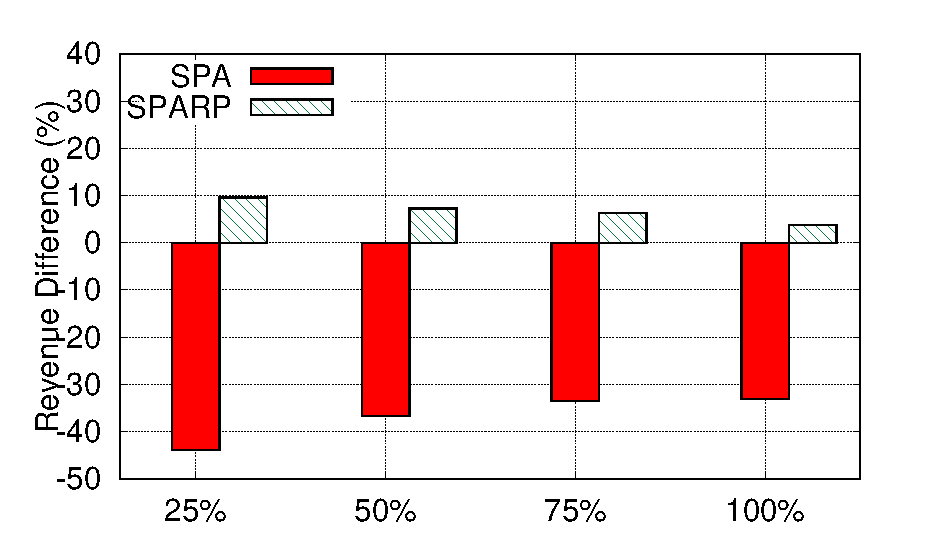
\includegraphics[width = 0.47\columnwidth]{fig/mad2revdiff}
    }
    \caption{\small{Comparing Relative Revenue of SPA \& SPARP Vs FPACB}}
    \label{fig:revdiff}
\end{figure}

In our next experiments, we changed the ratio of the drivers who bid untruthfully. As illustrated in \Cref{fig:cprev}, when no driver tries to manipulate the framework, FPACB generates more profit as compared to both SPA and SPARP (in this case there is no competitive bidding so FPACB works as the normal first-price auction scheme). However, as the percentage of untruthful drivers increases, the platform makes less revenue and when every driver is bidding competitively in FPACB, we notice that SPARP generates almost 10\% more revenue. In \Cref{sec:bidding} we proved that in theory, drivers can increase their utility by bidding untruthfully. To show this in practice, we observe in \Cref{tab:untruthful} that when drivers bid untruthfully, their average and median income per mile increases 20-25\%. At the same time, bidding untruthfully does not cost them losing many requests. We can see in \Cref{tab:untruthful} that the assigned requests for untruthful drivers is on average only 1 request less than truthful bidders.

\begin{figure}[h]
    \centering
    \subfigure[Untruthfull Drivers]{
        \label{fig:cp2rev}
        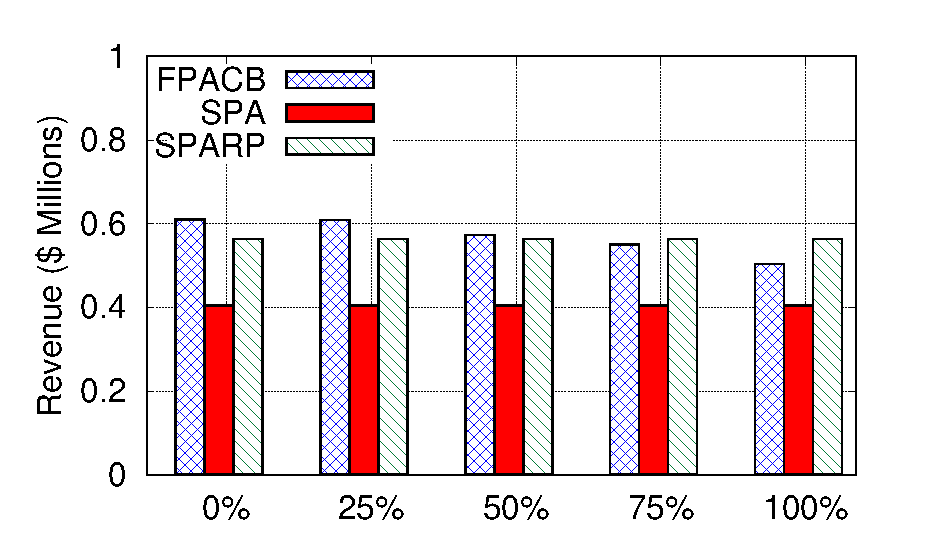
\includegraphics[width = 0.47\columnwidth]{fig/cp2rev}
    }
    \subfigure[Untruthfull Drivers]{
        \label{fig:cp2revdiff}
        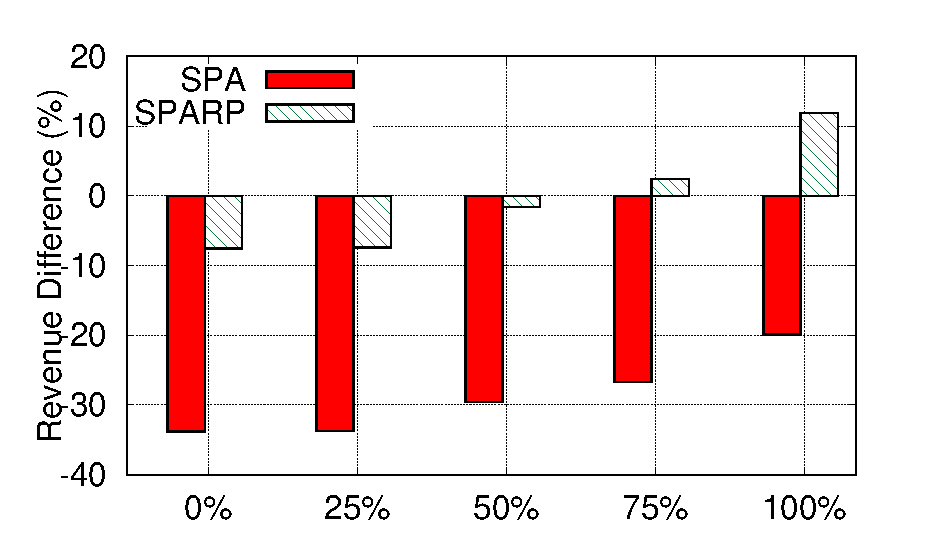
\includegraphics[width = 0.47\columnwidth]{fig/cp2revdiff}
    }
    \caption{\small{Comparing Relative Revenue of SPA \& SPARP Vs FPACB}}
    \label{fig:cprev}
\end{figure}

\begin{table}
  \centering
  \begin{tabular}{|c|c|c|c|c|}
    \hline
    \multicolumn{2}{|>{\columncolor{kugray5}}c|}{}&\multicolumn{3}{c|}{Untruthful Drivers (\%)}\\
    \arrayrulecolor{kugray5}
    \arrayrulecolor{black}
    \cline{3-5}
    \multicolumn{2}{|>{\columncolor{kugray5}}c|}{}&25\%&50\%&75\%\\
    \hline \hline
    \multirow{4}{*}{\begin{turn}{90}Truthful\end{turn}} &Assigned Requests (Average)&14.33&14.19&13.04\\
    \cline{2-5}
                         		&Assigned Requests (Median)&8&6&9\\
    \cline{2-5}
                         		&Income per Mile (Average)&\$1.00&\$1.00&\$1.00\\
    \cline{2-5}
                         		&Income per Mile (Median)&\$1.00&\$1.00&\$1.00\\
    \hline \hline
    \multirow{4}{*}{\begin{turn}{90}Untruthful\end{turn}}&Assigned Request (Average)&13.51&13.49&12.67\\
    \cline{2-5}
                         		&Assigned Requests (Median)&7&6&8\\
    \cline{2-5}
                         		&Income per Mile (Average)&\$1.24&\$1.25&\$1.24\\
    \cline{2-5}
                         		&Income per Mile (Median)&\$1.21&\$1.23&\$1.23\\
    \hline
  \end{tabular}
  \caption{Effects of Untruthful Bidding}
  \label{tab:untruthful}
\end{table}

The last set of our experiments focuses on how the accuracy of the prediction model can affect the utility of the drivers. For this experiment we compared the drivers' utilities when they predicted the number of drivers using LSTM with when they used LORE. To better explain the observed results, we distinguish between the cases where LORE overestimates and when it underestimates the number of drivers. As depicted in in \Cref{tab:accuracy}, when drivers overestimate, it causes them to take less risk in bidding. However, while this does not increase their chances of winning an auction, it does affect their average income per mile. With LSTM the drivers earn \textasciitilde25\% more by bidding competitively while when they overestimate the number of drivers, they only gain \textasciitilde15\% more than a driver who bids truthfully. On the other hand, when the drivers underestimate, their income per mile is up to 10\% higher as compared to using LSTM. However, this is the result of bidding much lower than their true valuation and as such they do not win many auctions. As shown in \Cref{tab:accuracy}, when drivers underestimate, they win about 50\% less auctions than when they predict more accurately.

\begin{table}
  \centering
  \begin{tabular}{|c|c|c|c|c|}
    \hline
    \multicolumn{2}{|>{\columncolor{kugray5}}c|}{}&\multicolumn{3}{c|}{Untruthful Drivers (\%)}\\
    \arrayrulecolor{kugray5}
    \arrayrulecolor{black}
    \cline{3-5}
    \multicolumn{2}{|>{\columncolor{kugray5}}c|}{}&25\%&50\%&75\%\\
    \hline \hline
    \multirow{4}{*}{\begin{turn}{90}LSTM\end{turn}}&Assigned Request (Average)&13.51&13.49&12.67\\
    \cline{2-5}
                         		&Assigned Requests (Median)&7&6&8\\
    \cline{2-5}
                         		&Income per Mile (Average)&\$1.24&\$1.25&\$1.24\\
    \cline{2-5}
                         		&Income per Mile (Median)&\$1.21&\$1.23&\$1.23\\
    \hline \hline
    \multirow{4}{*}{\begin{turn}{90}Over Est.\end{turn}} &Assigned Requests (Average)&14.01&13.98&12.91\\
    \cline{2-5}
                         		&Assigned Requests (Median)&7&6&8\\
    \cline{2-5}
                         		&Income per Mile (Average)&\$1.14&\$1.14&\$1.15\\
    \cline{2-5}
                         		&Income per Mile (Median)&\$1.11&\$1.12&\$1.11\\
    \hline \hline
    \multirow{4}{*}{\begin{turn}{90}Under Est.\end{turn}}&Assigned Request (Average)&7.51&7.39&8.81\\
    \cline{2-5}
                         		&Assigned Requests (Median)&5&4&5\\
    \cline{2-5}
                         		&Income per Mile (Average)&\$1.34&\$1.33&\$1.37\\
    \cline{2-5}
                         		&Income per Mile (Median)&\$1.32&\$1.31&\$1.32\\
    \hline

  \end{tabular}
  \caption{Effects of Prediction Accuracy}
  \label{tab:accuracy}
\end{table}


